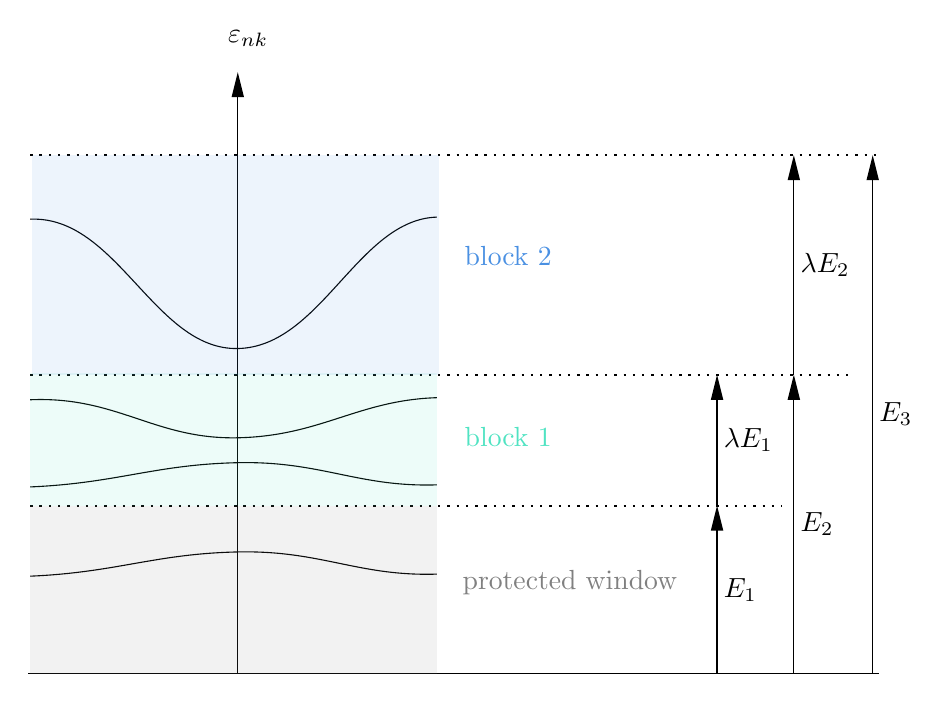
\begin{tikzpicture}[x=0.75pt,y=0.75pt,yscale=-1,xscale=1]
    %uncomment if require: \path (0,461); %set diagram left start at 0, and has height of 461
    
    %Straight Lines [id:da4347459027497955] 
    \draw    (59.96,416) -- (469.83,416) ;
    %Straight Lines [id:da41182270692893597] 
    \draw    (160.92,416.19) -- (160.92,128.19) ;
    \draw [shift={(160.92,126.19)}, rotate = 90] [fill={rgb, 255:red, 0; green, 0; blue, 0 }  ][line width=0.08]  [draw opacity=0] (12,-3) -- (0,0) -- (12,3) -- cycle    ;
    %Curve Lines [id:da05810441416458478] 
    \draw    (60.92,284) .. controls (102.83,282.19) and (120.83,303.19) .. (160.97,302.32) .. controls (201.1,301.45) and (218.83,284.19) .. (256.83,283) ;
    %Curve Lines [id:da4750454081922897] 
    \draw    (60.92,326) .. controls (102.83,324.19) and (120.83,315.19) .. (160.97,314.32) .. controls (201.1,313.45) and (218.83,326.19) .. (256.83,325) ;
    %Curve Lines [id:da23548696909292266] 
    \draw    (60.92,369) .. controls (102.83,367.19) and (120.83,358.19) .. (160.97,357.32) .. controls (201.1,356.45) and (218.83,369.19) .. (256.83,368) ;
    %Straight Lines [id:da41266249288678947] 
    \draw [line width=0.75]  [dash pattern={on 0.84pt off 2.51pt}]  (60.92,335) -- (422.83,335) ;
    %Straight Lines [id:da8456035131535149] 
    \draw [line width=0.75]  [dash pattern={on 0.84pt off 2.51pt}]  (60.92,272) -- (454.83,272) ;
    %Straight Lines [id:da48283445342794185] 
    \draw    (391.83,337) -- (391.83,416) ;
    \draw [shift={(391.83,335)}, rotate = 90] [fill={rgb, 255:red, 0; green, 0; blue, 0 }  ][line width=0.08]  [draw opacity=0] (12,-3) -- (0,0) -- (12,3) -- cycle    ;
    %Straight Lines [id:da27998896298251763] 
    \draw    (391.83,274) -- (391.83,335) ;
    \draw [shift={(391.83,272)}, rotate = 90] [fill={rgb, 255:red, 0; green, 0; blue, 0 }  ][line width=0.08]  [draw opacity=0] (12,-3) -- (0,0) -- (12,3) -- cycle    ;
    %Straight Lines [id:da1696859783248792] 
    \draw    (428.83,274) -- (428.83,416) ;
    \draw [shift={(428.83,272)}, rotate = 90] [fill={rgb, 255:red, 0; green, 0; blue, 0 }  ][line width=0.08]  [draw opacity=0] (12,-3) -- (0,0) -- (12,3) -- cycle    ;
    %Straight Lines [id:da8497758602589283] 
    \draw    (428.83,168.19) -- (428.83,272) ;
    \draw [shift={(428.83,166.19)}, rotate = 90] [fill={rgb, 255:red, 0; green, 0; blue, 0 }  ][line width=0.08]  [draw opacity=0] (12,-3) -- (0,0) -- (12,3) -- cycle    ;
    %Curve Lines [id:da35729452645998494] 
    \draw    (60.92,197) .. controls (102.83,195.19) and (120.83,260.19) .. (160.97,259.32) .. controls (201.1,258.45) and (218.83,197.19) .. (256.83,196) ;
    %Straight Lines [id:da7747060246021067] 
    \draw [line width=0.75]  [dash pattern={on 0.84pt off 2.51pt}]  (60.92,166.19) -- (469.83,166.19) ;
    %Straight Lines [id:da3642603327182674] 
    \draw    (466.83,168.19) -- (466.83,416) ;
    \draw [shift={(466.83,166.19)}, rotate = 90] [fill={rgb, 255:red, 0; green, 0; blue, 0 }  ][line width=0.08]  [draw opacity=0] (12,-3) -- (0,0) -- (12,3) -- cycle    ;
    %Shape: Rectangle [id:dp8763269535201674] 
    \draw  [draw opacity=0][fill={rgb, 255:red, 128; green, 128; blue, 128 }  ,fill opacity=0.1 ] (60.92,335) -- (256.83,335) -- (256.83,416) -- (60.92,416) -- cycle ;
    %Shape: Rectangle [id:dp4702244212893545] 
    \draw  [draw opacity=0][fill={rgb, 255:red, 80; green, 227; blue, 194 }  ,fill opacity=0.1 ] (60.92,271.19) -- (256.83,271.19) -- (256.83,335) -- (60.92,335) -- cycle ;
    %Shape: Rectangle [id:dp6975366095055684] 
    \draw  [draw opacity=0][fill={rgb, 255:red, 74; green, 144; blue, 226 }  ,fill opacity=0.1 ] (61.96,166.19) -- (257.87,166.19) -- (257.87,272) -- (61.96,272) -- cycle ;
    
    % Text Node
    \draw (268,365) node [anchor=north west][inner sep=0.75pt]  [color={rgb, 255:red, 128; green, 128; blue, 128 }  ,opacity=1 ] [align=left] {protected window};
    % Text Node
    \draw (155,105) node [anchor=north west][inner sep=0.75pt]    {$\varepsilon _{nk}$};
    % Text Node
    \draw (393.83,375.5) node [anchor=west] [inner sep=0.75pt]    {$E_{1}$};
    % Text Node
    \draw (393.83,303.5) node [anchor=west] [inner sep=0.75pt]    {$\lambda E_{1}$};
    % Text Node
    \draw (430.83,344) node [anchor=west] [inner sep=0.75pt]    {$E_{2}$};
    % Text Node
    \draw (430.83,219.09) node [anchor=west] [inner sep=0.75pt]    {$\lambda E_{2}$};
    % Text Node
    \draw (468.83,291.09) node [anchor=west] [inner sep=0.75pt]    {$E_{3}$};
    % Text Node
    \draw (269,296) node [anchor=north west][inner sep=0.75pt]  [color={rgb, 255:red, 80; green, 227; blue, 194 }  ,opacity=1 ] [align=left] {block 1};
    % Text Node
    \draw (269,209) node [anchor=north west][inner sep=0.75pt]  [color={rgb, 255:red, 74; green, 144; blue, 226 }  ,opacity=1 ] [align=left] {block 2};
    
    
    \end{tikzpicture}
    